\documentclass[a4paper]{article}
\usepackage[a4paper, total={6in, 9in}]{geometry}
\usepackage{graphicx}
%\setlength{\parindent}{0cm}
\usepackage{amsmath}
\usepackage{amssymb}
\usepackage{graphicx}
\usepackage{hyperref}
\usepackage{enumitem} 
\usepackage{hyperref}
\usepackage{graphicx}
\usepackage[parfill]{parskip}
\usepackage{lingmacros}
\usepackage{tree-dvips}
\usepackage{pythonhighlight}
\usepackage{graphicx}
\usepackage{caption}
\usepackage{subcaption}
\usepackage[export]{adjustbox}
\graphicspath{ {/home/user/Desktop/Cover Page} }
\begin{document}


% TITLE PAGE

\begin{titlepage}

\raggedleft

\includegraphics[scale=0.4]{Logo.png}\\

\vspace{3cm}
\begin{center}
\newcommand{\HRule}{\rule{\linewidth}{0.5mm}}
\textsc{\Large MATH3001: Project in Mathematics}\\[2.0mm]
\textsc{\Large School of Mathematics}\\[2.0mm]
\vspace{0.5cm}

	\HRule\\[0.4cm]

	{\huge\bfseries Using Random Numbers to Solve Problems in Maths and Physics}\\[0.4cm] 

	\HRule\\[1.5cm]

		\begin{minipage}{0.4\textwidth}
		\begin{flushleft}
			\large
			\textit{Author:}\\
			\text{Eleanor Sleightholm} \\
			\text{(201214895)}
		\end{flushleft}
	\end{minipage}
	~
	\begin{minipage}{0.4\textwidth}
		\begin{flushright}
			\large
			\textit{Supervisors:}\\
			\text{Dr Oliver Harlen} \\
			\text{Dr Mike Evans}
		\end{flushright}
	\end{minipage}
\mbox{}
\vfill
\text{December 11, 2020}

\end{center}
\end{titlepage}

% TABLE OF CONTENTS

\tableofcontents

% STARTING THE REPORT
\newpage
%\section{Interactions and Phase Transitions}
\parskip = \baselineskip
\section{General Introduction}

Talk about Monte Carlo methods - why they're useful, etc

\section{Molecules in Materials - Boltzmann Distribution}

There is one particular application in which high-dimensional Monte Carlo sampling is very widely and successfully used: to model the behaviour of atoms and molecules within a material such as a fluid.

Talk about statistical mechanics, the idea behind the boltzmann distribution - keep it to 1 or 2 pages.

\section{The Ising Model}
\parskip = \baselineskip
The Ising Model, named after Ernst Ising$^{[1]}$, is a mathematical model of ferromagnetism in statistical mechanics. Ferromagnetism arises when a collection of atomic spins align such that their associated magnetic moments all point in the same direction, yielding a net magnetic moment. The Ising Model is the simplest theoretical description of ferromagnetism. This model was invented by Wilhelm Lenz in 1920 and subsequently named after Ernst Ising who chose the model as a subject of his doctoral dissertation in 1925.
\parskip = \baselineskip

The Ising model works by representing each atom by an arrow that can point either up or down. This arrow
is also known as a “spin” and corresponds to the direction of the atom’s own magnetic moment. The model considers a lattice of size $N$ with spins at each lattice site that can
take only two values, ±$1$ (up or down respectively). We use the variable $\sigma_{i}$ to denote the
direction of the ith spin, with $\sigma_{i}$ = $+1$ representing up and  $\sigma_{i}$ = $-1$ representing down.
This lattice can be visually represented like in Figure 1 where blue arrows represent up spins ($+1$) and
red arrows represent down spins ($-1$).

\begin{figure}[h]
\centering
\begin{subfigure}{0.3\textwidth}
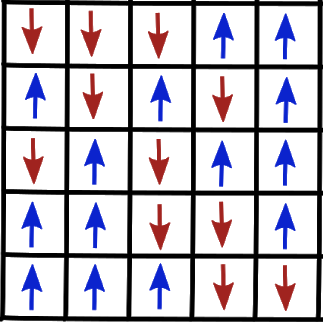
\includegraphics[width=1\linewidth]{lattice.png} 
\caption{A Lattice of Size 5}
\label{fig:subim1}
\end{subfigure}
\hspace{1cm}
\begin{subfigure}{0.2\textwidth}
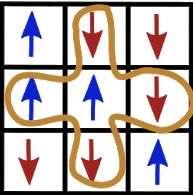
\includegraphics[width=1.1\linewidth]{nearestneighbours.png}
\vspace{0.6cm}
\caption{$<i, j>$}
\label{fig:subim2}
\end{subfigure}
\caption{Lattice Properties}
\label{fig:image2}
\end{figure}




Thus, if $N$ atoms are arranged on a lattice, like in Figure 1, then a state of the system can be represented by an array of $N$ values, each equal to ±$1$.
The total energy of the system is written:

\begin{equation}
E = -J\sum_{<i,j>} \sigma_{i}\sigma_{j} \, - \mu h\sum_{i} \sigma_{i} \,
\end{equation}

where $<i,j>$ denotes that the summation is over the values of $i$ and $j$ that correspond to nearest neighbour spins; pairs of spins that are positioned next to each other on the lattice. This can be seen in Figure 2. Two neighbouring up spins or two neighbouring down spins have $E_{pair} = 1$ and two spins anti-aligned have $E_{pair} = -1$. $J$, $\mu$ and $h$ are parameters of the model where $J$ refers to the exchange energy and $\mu$ refers to the atomic magnetic moment.

Using this equation, we are able to understand physical aspects of the Ising model. We notice that the first summation shows that the overall energy is lowered when neighbouring spins are aligned. Subsequently, the overall energy is heightened when neighbouring spins are anti-aligned. From this we can deduce that the Boltzmann law gives preference to parallel alignment of neighbours. Similarly, the second summation will have lowest energy when spins in the lattice are pointing up ($\sigma_{i} = 1$). Thus, for the energy of the system to be at its lowest, all spins must be pointing upwards. 

\subsection{The Metropolis Algorithm for the Ising Model}

Adopting the Monte Carlo approach to the Ising model allows for visualisations and analysis of the overall system. The main steps for the Metropolis algorithm for the Ising model is as follows,

\begin{description}[font=$\bullet$~\normalfont\scshape]
\item [Step 1] Start in an initial configuration of $N$ spins.
\item [Step 2] Choose a random lattice site and flip the spin, $\sigma_{i}$ located there.
\item [Step 3] Calculate the change in energy $\triangle{E_{i}}$.
\item [Step 4] If $\triangle{E_{i,j}} < 0$, accept the move. \\ Otherwise, accept the move with probability, $\exp \Big( - \frac{\triangle{E_{i}}\textsubscript{i}}{k\textsubscript{B} T}\Big)$.
\item [Step 5] Repeat Steps 2 to 4 until the system reaches a equilibrium.
\end{description}

\subsection{Two Dimensional Ising Model}

We consider a two-dimensional system with no magnetic field, this is called $spontaneous$ $magnetisation$. The overall energy is now defined as,
\begin{align}
E = -J\sum_{<i,j>} \sigma_{i}\sigma_{j} \
\end{align}
Using this, we can observe the behaviour between energy and temperature, as can be seen in Figure 3. Temperature induces motion into the system by allowing spins to alternate their signs. Temperature has the influence of moving the system into different spin configurations over time. Taking into consideration that the probability of finding the system in a specific state $i$ is proportional to the Boltzmann factor defined earlier, 
 \begin{align*} 
p\textsubscript{i} = A\exp \Big( - \frac{E\textsubscript{i}}{k\textsubscript{B} T}\Big)
\end{align*}

where ${k\textsubscript{B}}$ is the Boltzmann constant, $T$ is the temperature and $E\textsubscript{i}$ is the energy of the state. From this we can deduce that as the temperature increases, states with increasing energies become more populated. Similarly, at lower temperatures, the spin configurations will be near the lowest-energy configurations; where all the spins are aligned, either up or down. This is depicted in Figure 3 where the energy increases as temperature increases.   

\begin{figure}[h]
\centering
\begin{subfigure}{0.5\textwidth}
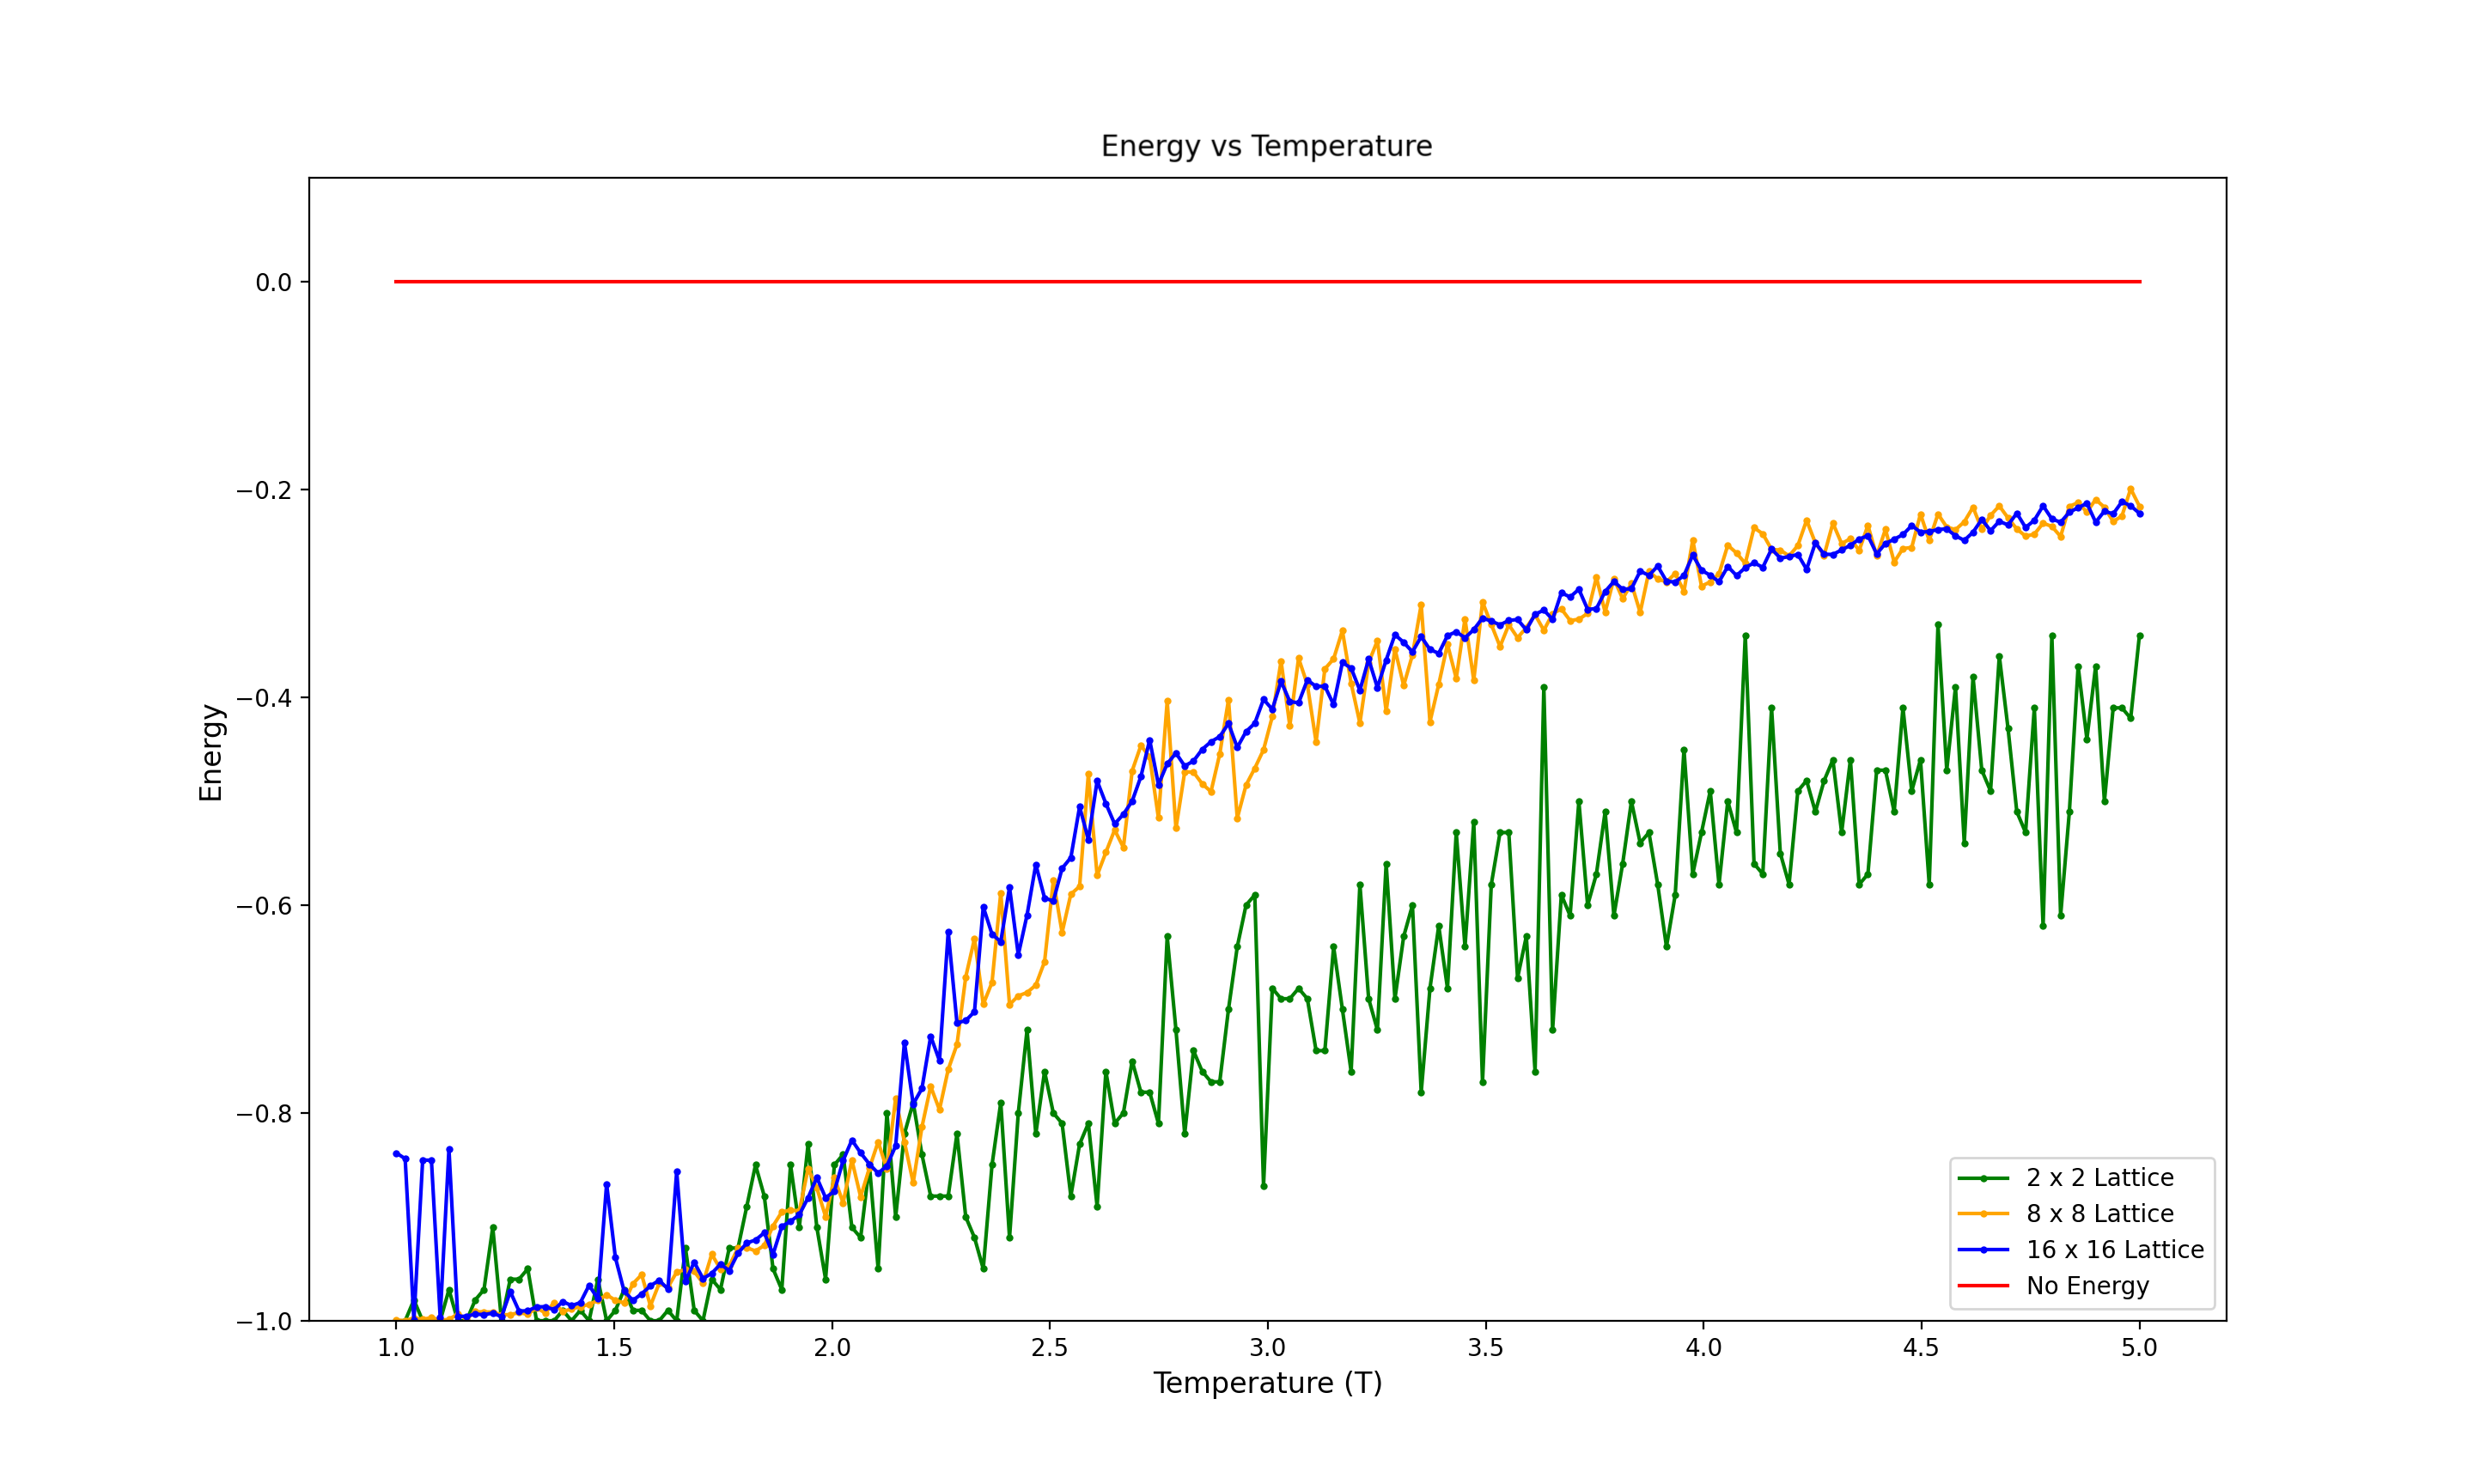
\includegraphics[width=1\linewidth]{energy vs temp.png} 
\caption{Energy vs Temperature}
\label{fig:subim1}
\end{subfigure}
\begin{subfigure}{0.425\textwidth}
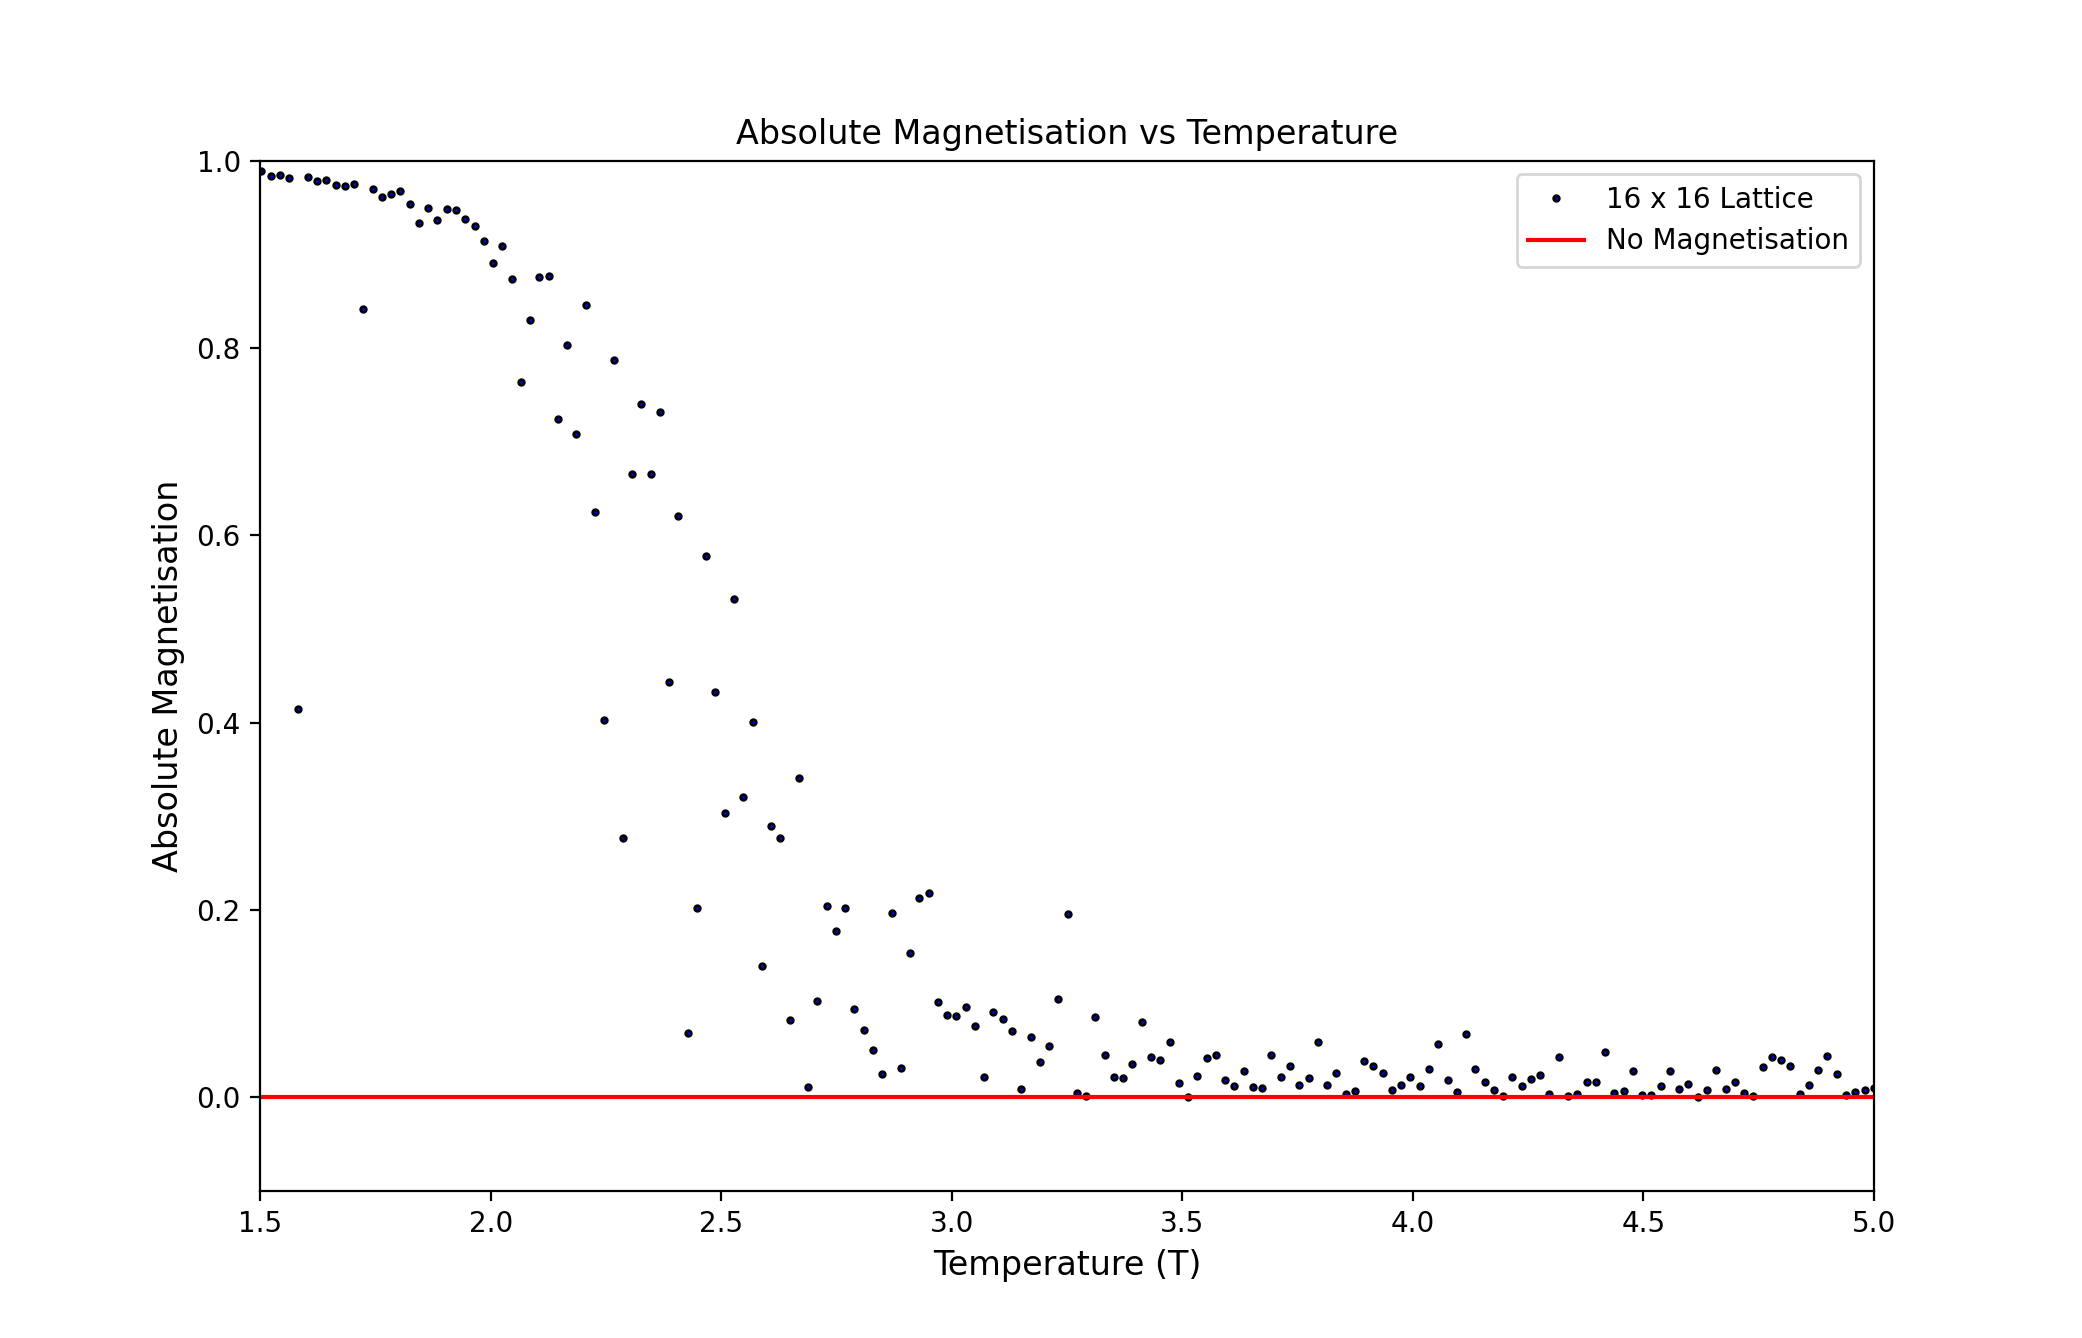
\includegraphics[width=1.1\linewidth,left]{mag vs temp.png}
\caption{Absolute Magnetisation vs Temperature}
\label{fig:subim2}
\end{subfigure}
\caption{Simulations of Energy and Magnetism vs Temperature}
\label{fig:image2}
\end{figure}

As the temperature increases, the net energy decreases but remains negative. This implies that more spins are aligned in the same direction. As stated above, we expect this phenomenon during lower temperatures. In addition, the decreasing net energy is also expected as the system of spins becomes increasingly more random as temperature is increased.

Treating each spin as a micro-magnet, the mean magnetisation of the system can be defined as,
\begin{align*}
M = \frac{1}{N}\sum_{i}^{N} \sigma_{i} \
\end{align*}
From this it can be deduced that at zero temperature, the magnetisation is 1. It follows that this is optimal magnetisation of the system and as temperature increases, the magnetisation of the system decreases. This can be depicted in Figure 4.

In Figure 3, the energy spikes and in Figure 4, the absolute magnetisation drops drastically down to 0. Since the absolute magnetisation of the system drops to 0, this represents a complete loss of magnetism. Thus, the system has undergone a second order phase transition at a critical temperature $T_{c}$. The system magnetises at temperatures less than $T_{c}$, this state is called ferromagnetic or ordered. The system is then considered paramagnetic or disordered for temperatures greater than $T_{c}$. By observing Figures 3 and 4, we estimate the critical temperature to be between 2 and 2.5.

During a phase transition, we expect the specific heat capacity of the system to increase. We can simulate a specific heat capacity versus temperature plot for a given lattice and observe whether the change in heat capacity occurs at the observed critical temperature.

Using the standard result in equilibrium statistical thermodynamics, heat capacity is defined as,
\begin{align*}
C = \frac{\sigma_{E}^2}{k_{B}T^2}
\end{align*}
where $\sigma_{E}$ denotes the standard deviation of fluctuations in energy. We can calculate $\sigma_{E}$ as follows, 
\begin{align*}
\sigma_{E}^2 =  {\langle E^2\rangle} - {\langle E\rangle ^2}
\end{align*}
 where $E$ is defined in equation (2).
 
Now we have an equation for the specific heat capacity, we can plot this against temperature, as seen in Figure 5. 

\begin{figure}[h!]
  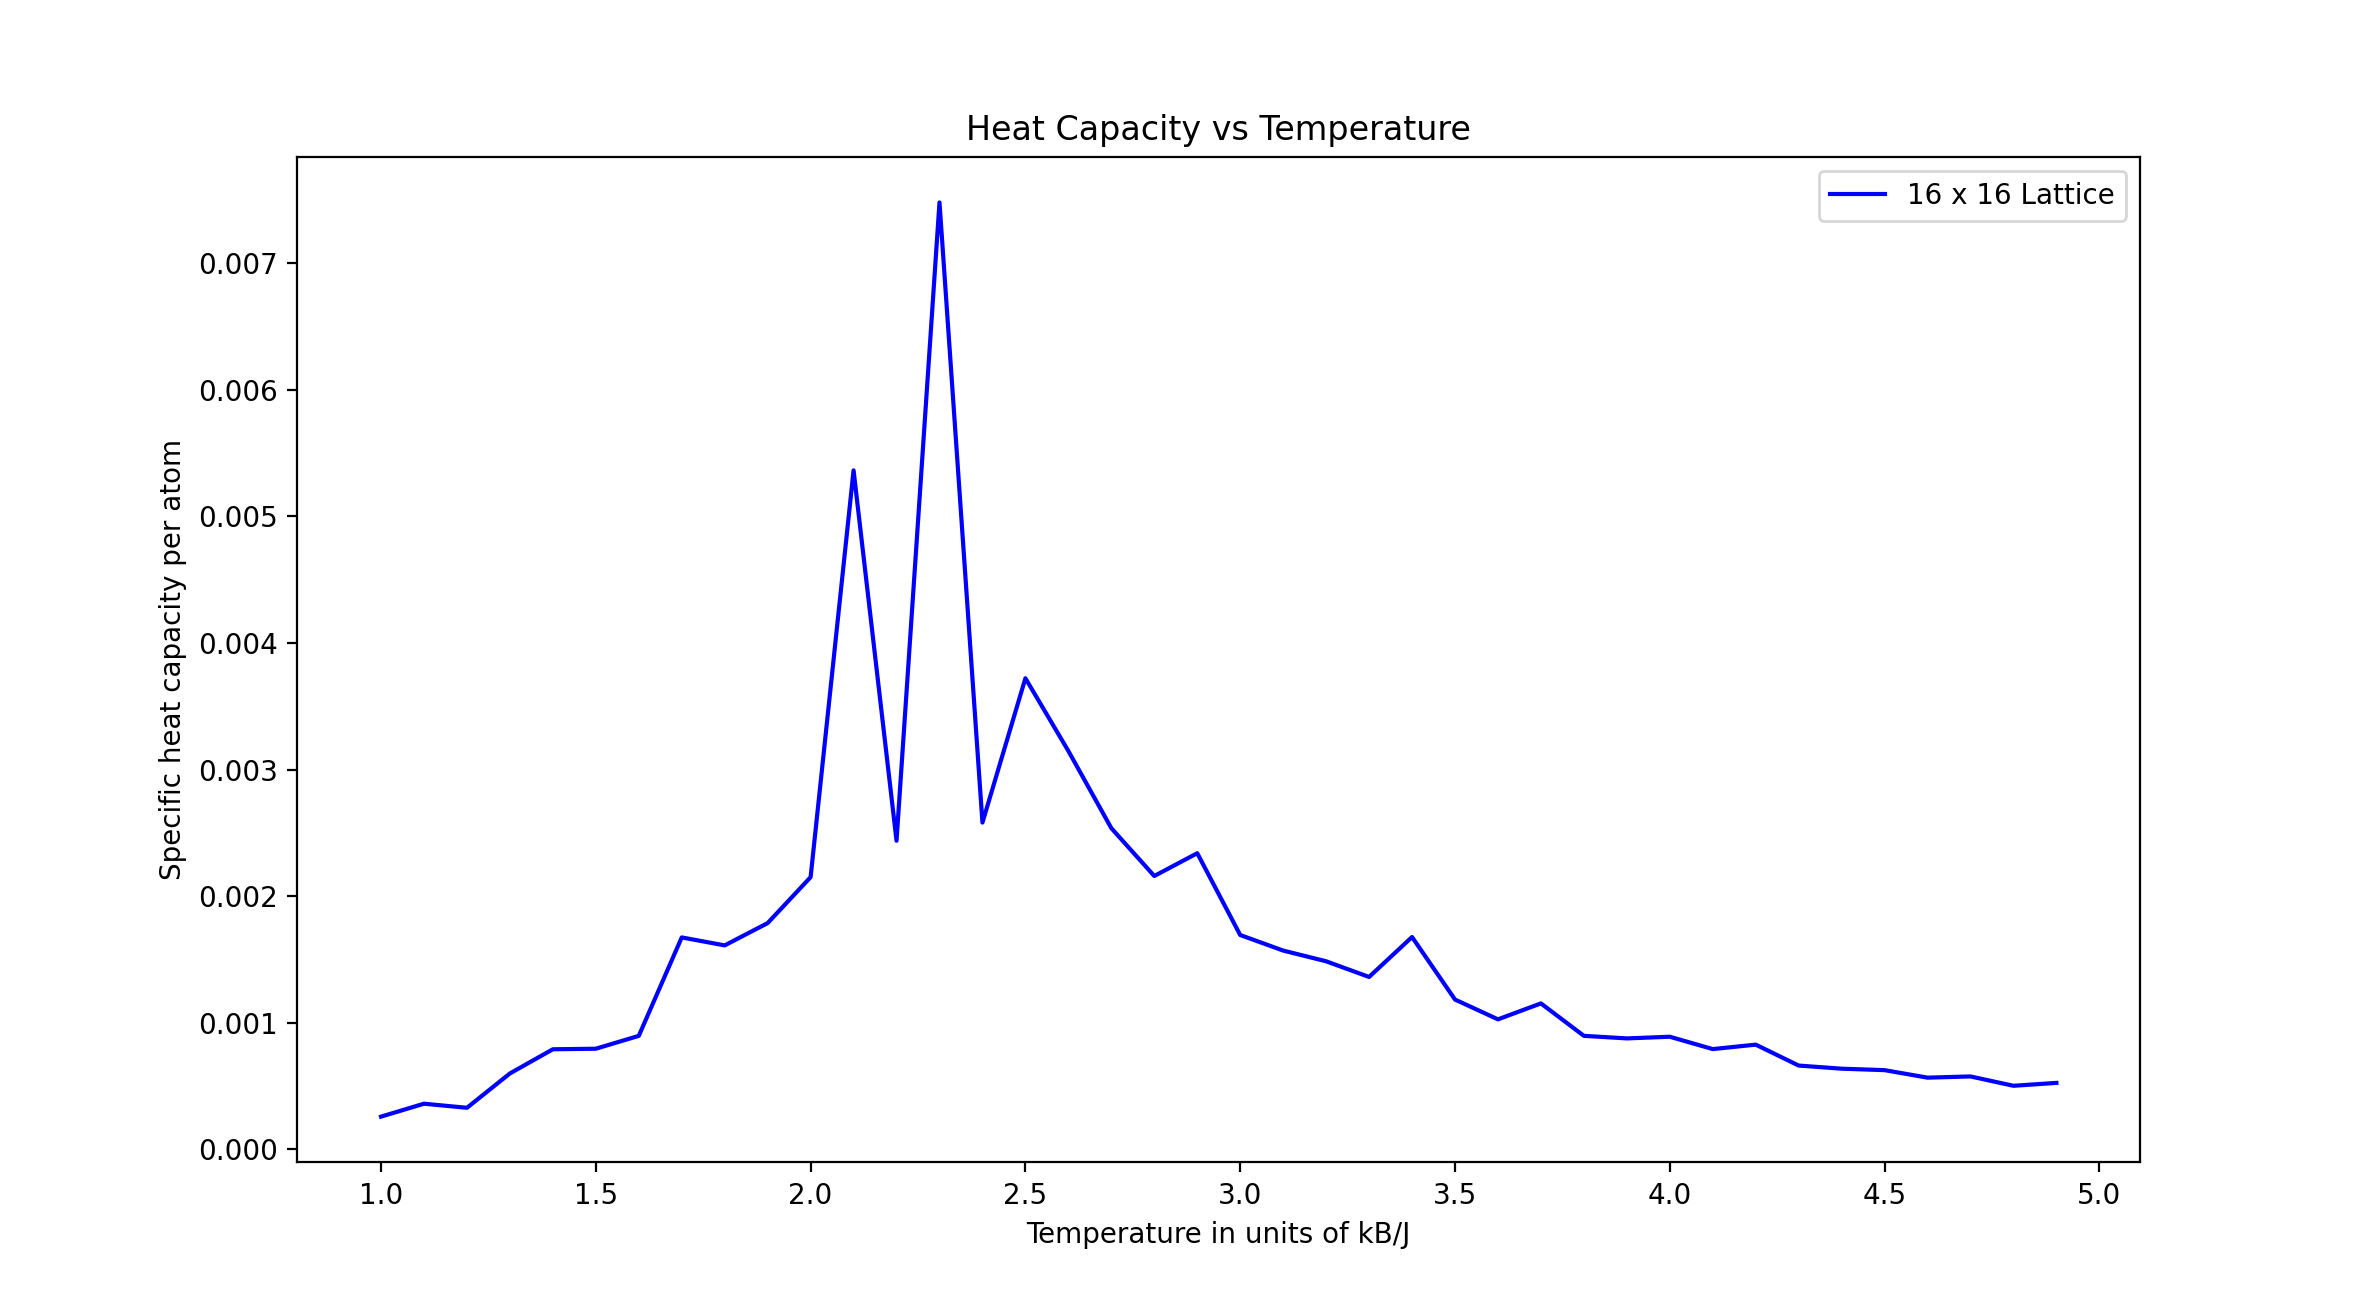
\includegraphics[scale=0.3, center]{heat capacity vs temperature.png}
  \caption{Heat Capacity vs Temperature}
  \label{fig:estimated_mean}
\end{figure} 

It is clear that we see a large increase or 'spike' in the heat capacity around 2 and 2.5. This sharp increase denotes the system going through its phase transition. Thus, we can conclude that the system underwent a phase transition between these temperatures. 

Although we can observe an estimated critical temperature, we move onto calculating this temperature analytically. With the analytically calculated critical temperature, we can observe the system for temperatures above, equal and below this temperature.

\subsection{Critical Temperature, $T_{c}$, of the 2D Ising Model}

We now adopt an analytical approach for calculating this critical temperature in two dimension. For a one dimension lattice with no external magnetic field, it can be shown that the critical temperature, $T_{c}$, is 0. 

In 1944, Theoretical Physicist, Lars Onsager, obtained the exact, analytical solution of the two-dimensional Ising model. [ Input a reference ]. Since this time, there has been no exact solution to the Ising model with an external magnetic field or in higher dimensions.

Onsager's solution shows that there exists a second order phase transition at a critical value of,
\begin{align*}
\frac{k_{B}T_{c}}{J} = \frac{2}{\log(1 + \sqrt{2})}
\end{align*}
Generally, with alternating $k_{B}$ and $J$, the critical temperature becomes, 
\begin{align*}
T_{c} = \frac{2J}{\log(1 + \sqrt{2})k_{B}} \approx \frac{2.269185J}{k_{B}}
\end{align*}
Like in our python code, we set $k_{B}$ and $J$ to equal 1 in order to simplify this calculation. Thus, the critical temperature for our plots becomes, 
\begin{align*}
T_{c} = \frac{2}{\log(1 + \sqrt{2})} \approx 2.269185...
\end{align*}
This value of the critical temperature aligns with Figures 3 and 4. Figure 3 illustrates a sharp increase in energy while Figure 4 shows a sharp decrease in magnetisation around the critical temperature. These figures clearly illustrate a second order phase transition around the critical temperature.

Extending this further, we can observe how the system behaves for temperatures above, equal or below the critical temperature. Recall that we are considering a system with no external magnetic field.

\subsubsection{$T < T_{c}$}

For $T < T_{c}$, the system is in a low temperature phase. Thus, we expect a dominance of one directional spin ($\sigma_{i} \pm 1$) with fluctuations of the opposing directional spin in small clusters or points, as can be seen in Figure 5(a). These small clusters will increase in size as T approaches the temperature at which a second order phase transition begins, $T \rightarrow T_{c}$.

\begin{figure}[h]
\centering
\begin{subfigure}{0.4\textwidth}
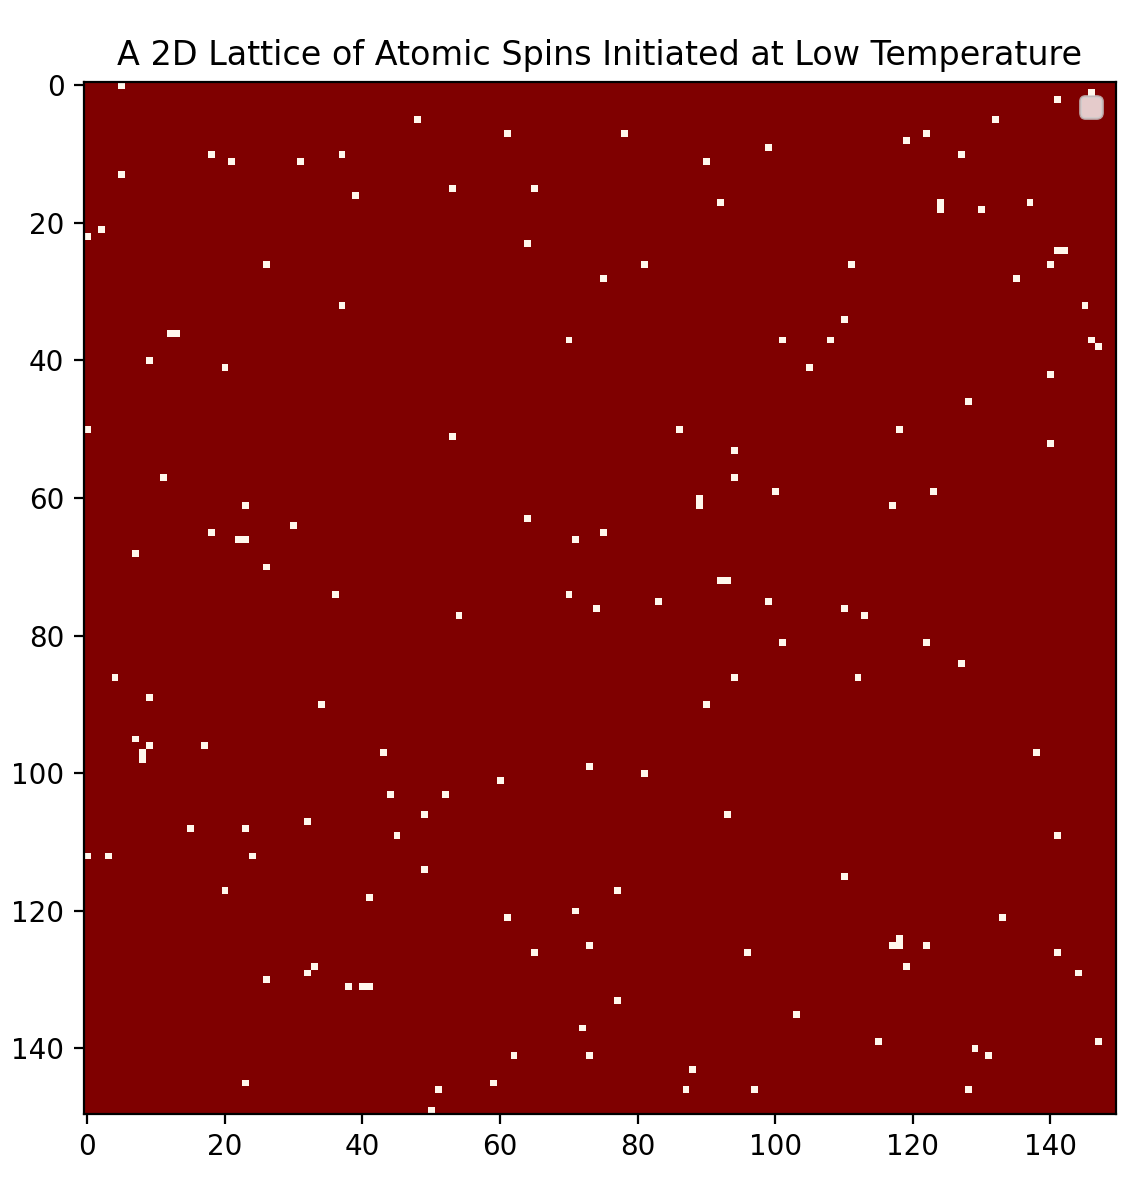
\includegraphics[width=1\linewidth]{2D Low Temperature.png} 
\caption{2D Lattice of Atomic Spins}
\label{fig:subim1}
\end{subfigure}
\begin{subfigure}{0.5\textwidth}
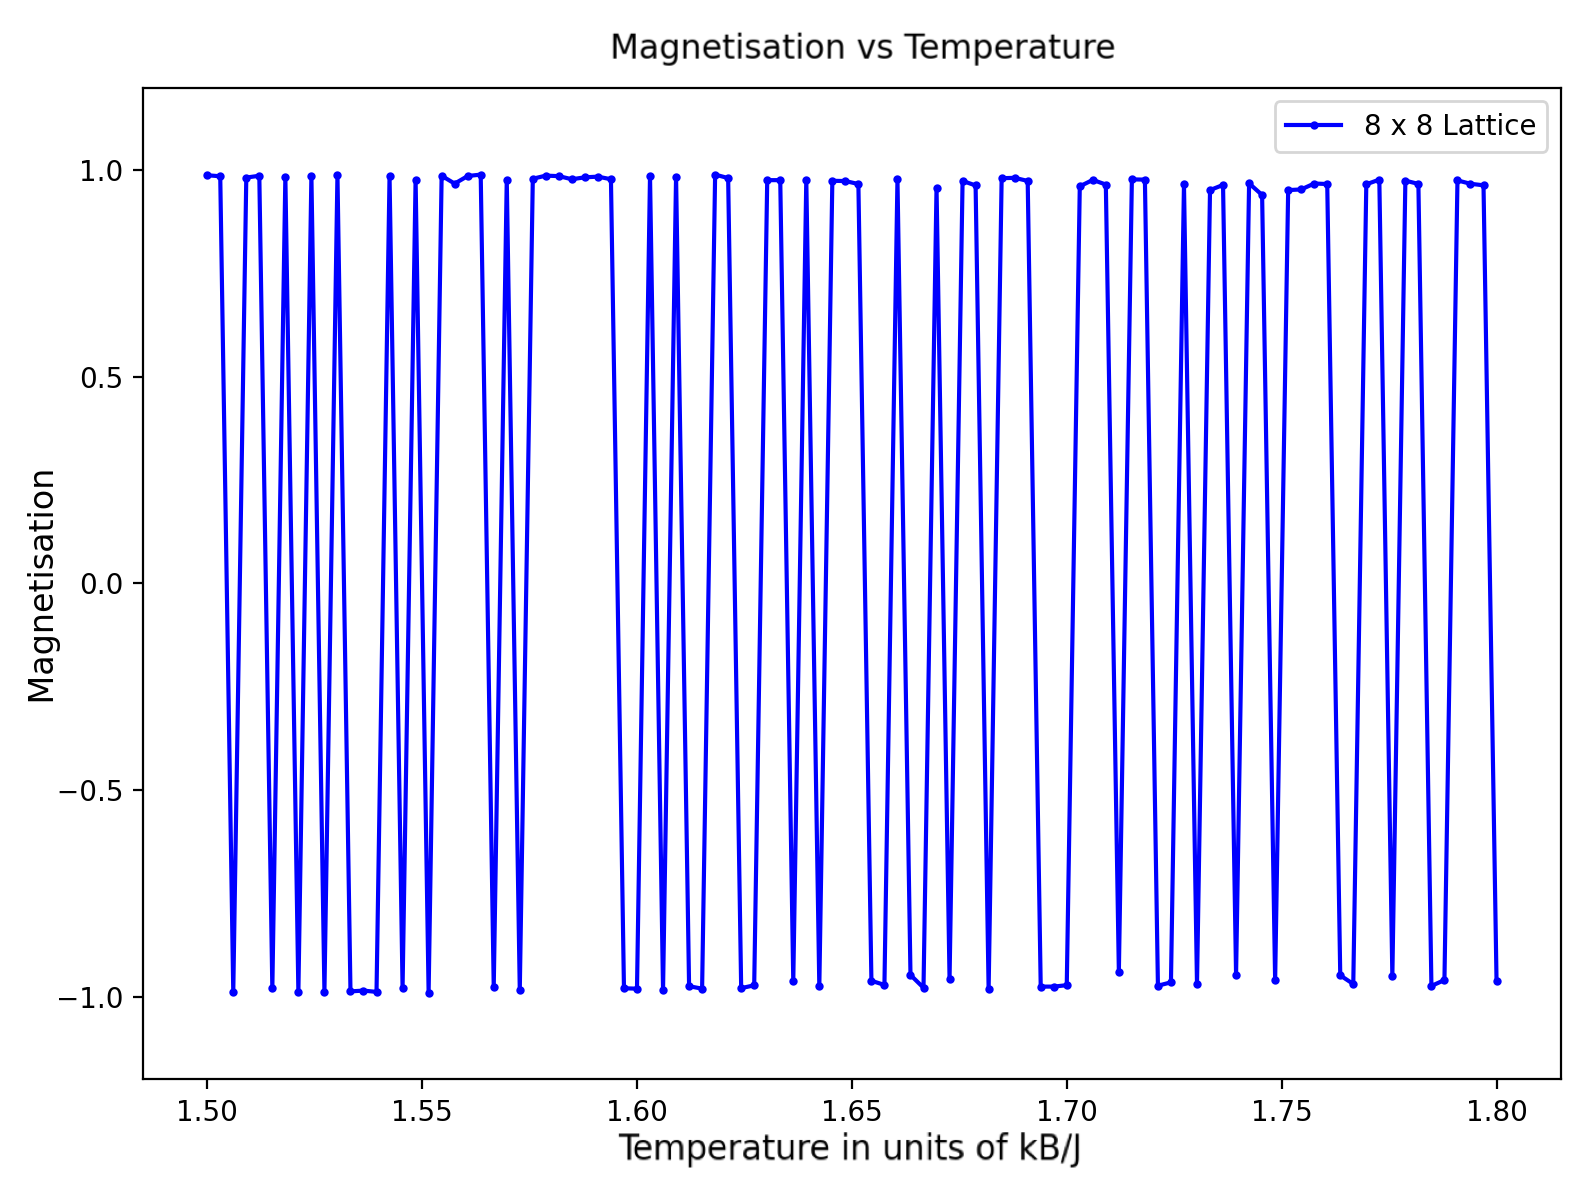
\includegraphics[width=1.1\linewidth,left]{mag vs temp for low temp.png}
\caption{Magnetisation vs Temperature}
\label{fig:subim2}
\end{subfigure}
\caption{2D Ising Model at Low Temperature}
\label{fig:image2}
\end{figure}

Figure 5(b) reiterates that magnetisation is at its optimal during lower temperatures. The figure illustrates that magnetisation only occurs at $\pm{1}$. From this, we can deduce that a system at low temperature will take less steps and time to reach equilibrium by the Monte Carlo Metropolis Algorithm.

\subsubsection{$T \approx T_{c}$}

\begin{figure}[h]
\centering
\begin{subfigure}{0.4\textwidth}
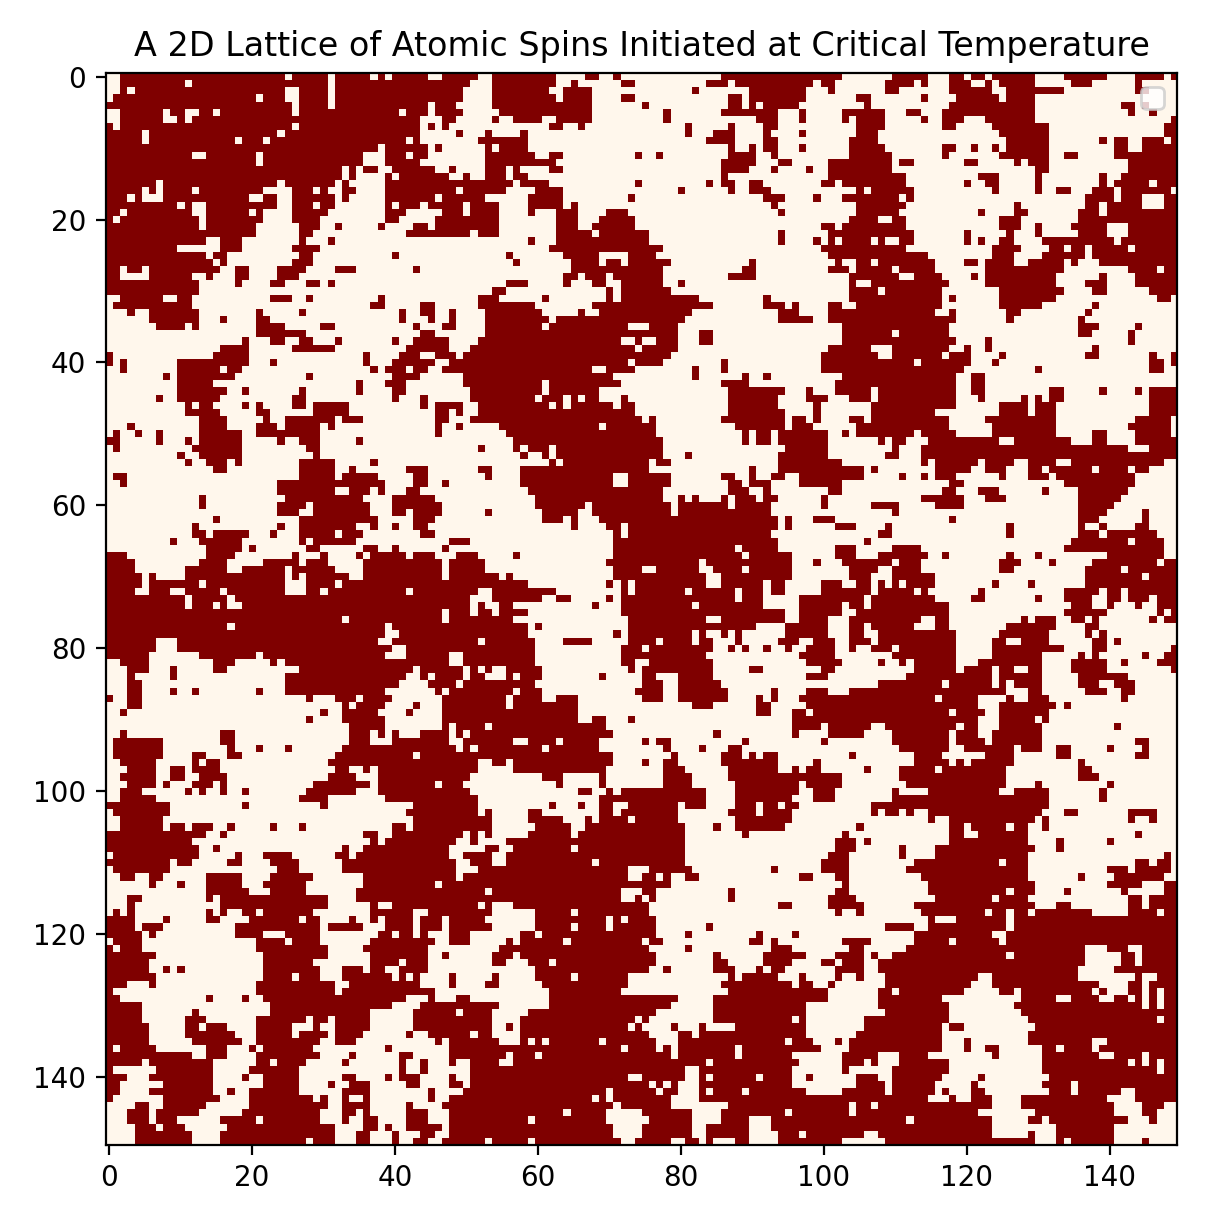
\includegraphics[width=1\linewidth]{2D Lattice Critical Temp.png} 
\caption{2D Lattice of Atomic Spins}
\label{fig:subim1}
\end{subfigure}
\begin{subfigure}{0.5\textwidth}
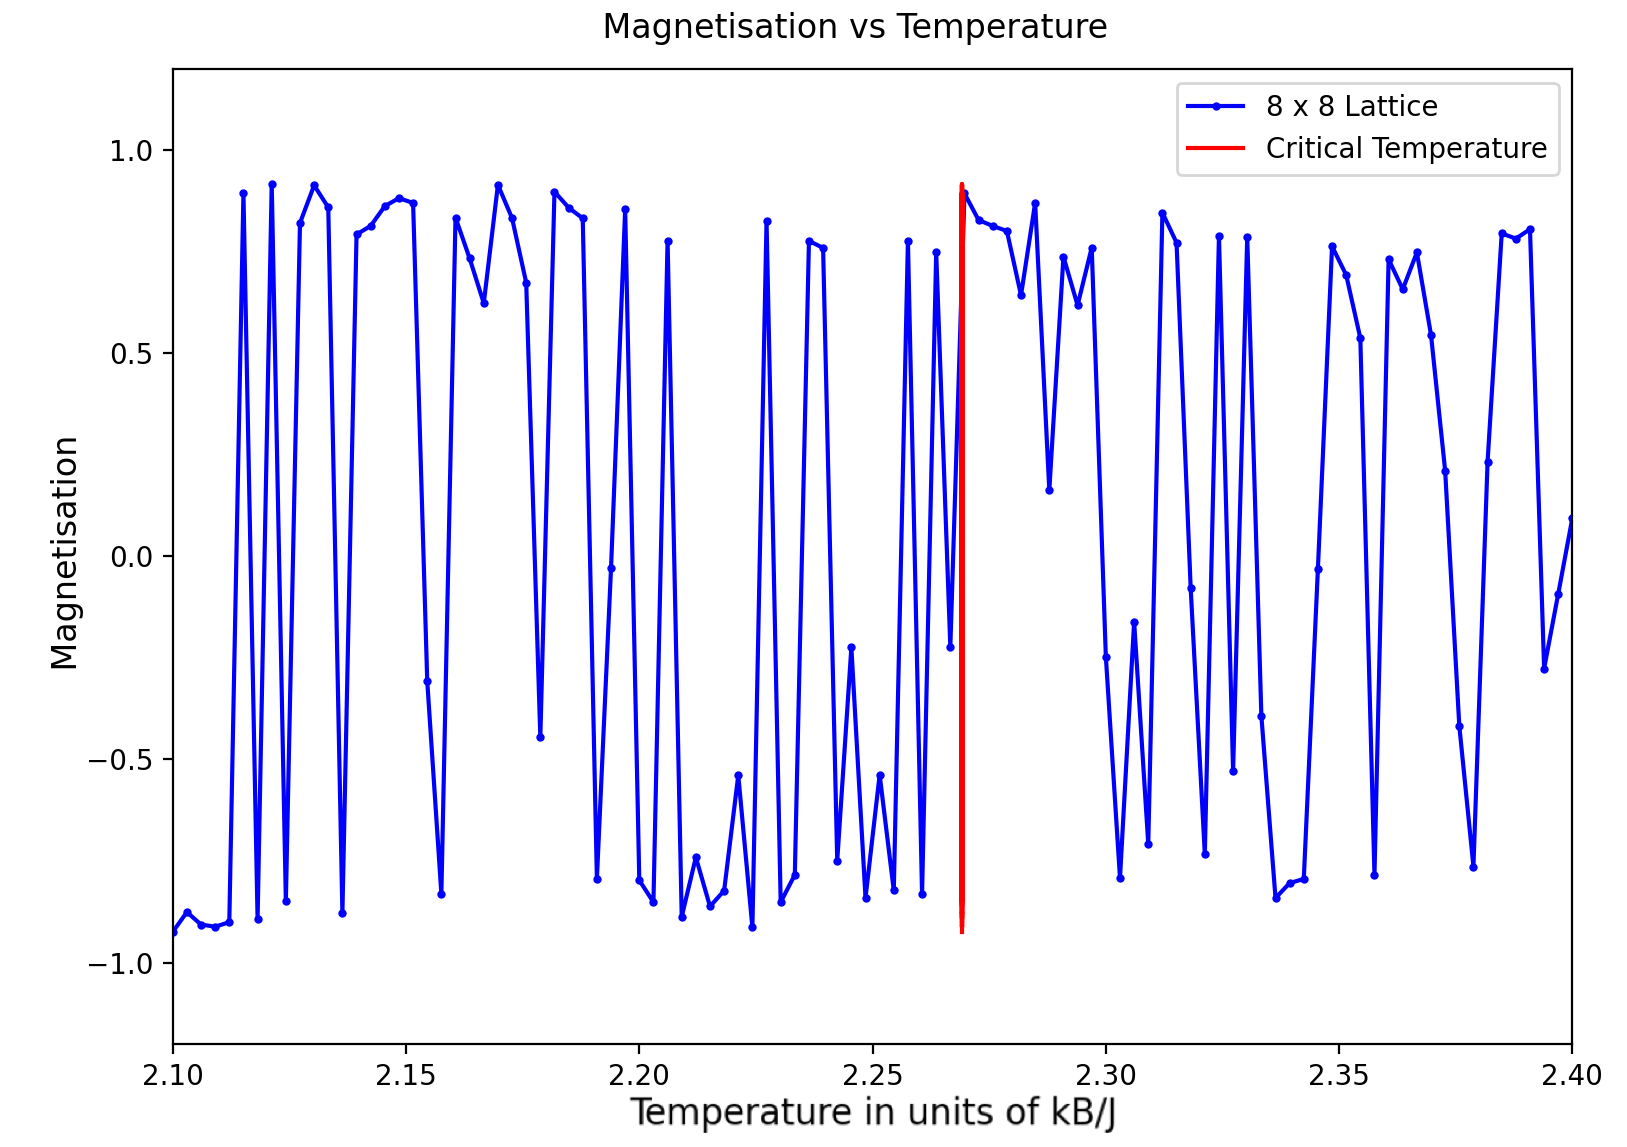
\includegraphics[width=1.1\linewidth,left]{mag vs temp critical temp.png}
\caption{Magnetisation vs Temperature}
\label{fig:subim2}
\end{subfigure}
\caption{2D Ising Model at Critical Temperature}
\label{fig:image2}
\end{figure}

At critical temperature, we expect to observe the system undergoing the second order phase transition, as predicted by Onsager's solution. During this phase transition, fluctuations in the spins will occur with no clear dominance of one spin, as depicted in Figure 7(a).

The magnetisation of the system is expected to fluctuate as a result of the fluctuations in spins. This is illustrated in Figure 7(b) where the magnetisation of the system differs around the critical temperature. 

Starting a system with temperature at its critical temperature will result in signs of decay in the alignment as the system passes through iterations of the Metropolis Algorithm. The system can reach equilibrium but due to the declining magnetism, the system cannot maintain equilibrium.

\subsubsection{$T > T_{c}$}

At high temperatures, we know that the system's energy will increase and thus, create an imbalance between the alignment of spins. This has already been depicted in Figure 3. Owing to this, we expect the system to appear random with no dominance of one spin and no obvious patterns. This observation can be shown in Figure 8(a). 

\begin{figure}[h]
\centering
\begin{subfigure}{0.37\textwidth}
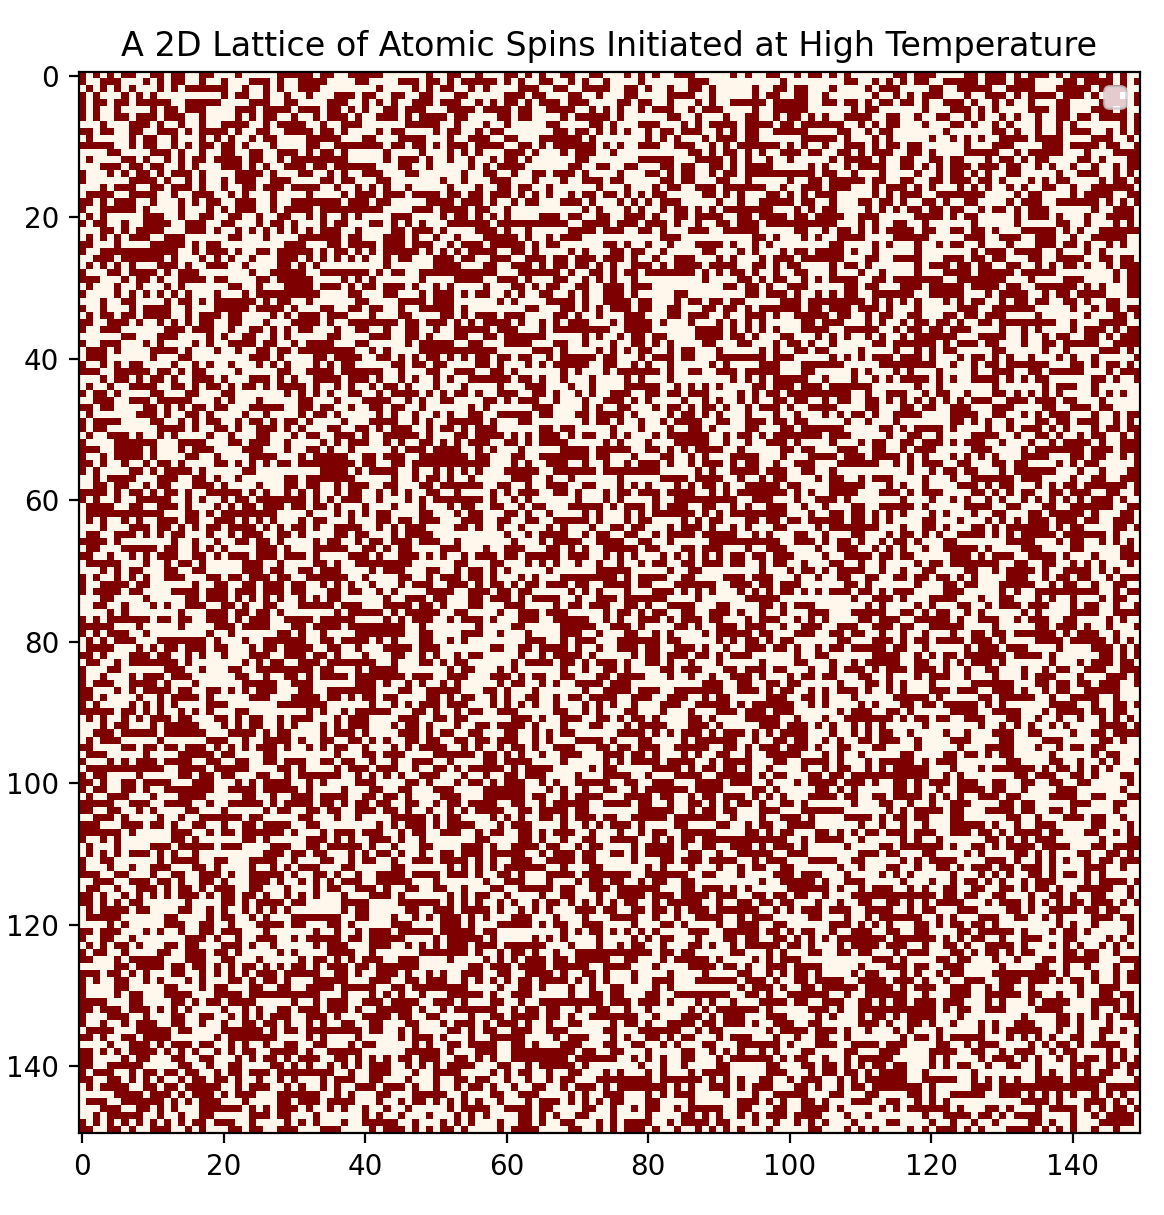
\includegraphics[width=1\linewidth]{2D Lattice High Temperature.png} 
\caption{2D Lattice of Atomic Spins}
\label{fig:subim1}
\end{subfigure}
\begin{subfigure}{0.5\textwidth}
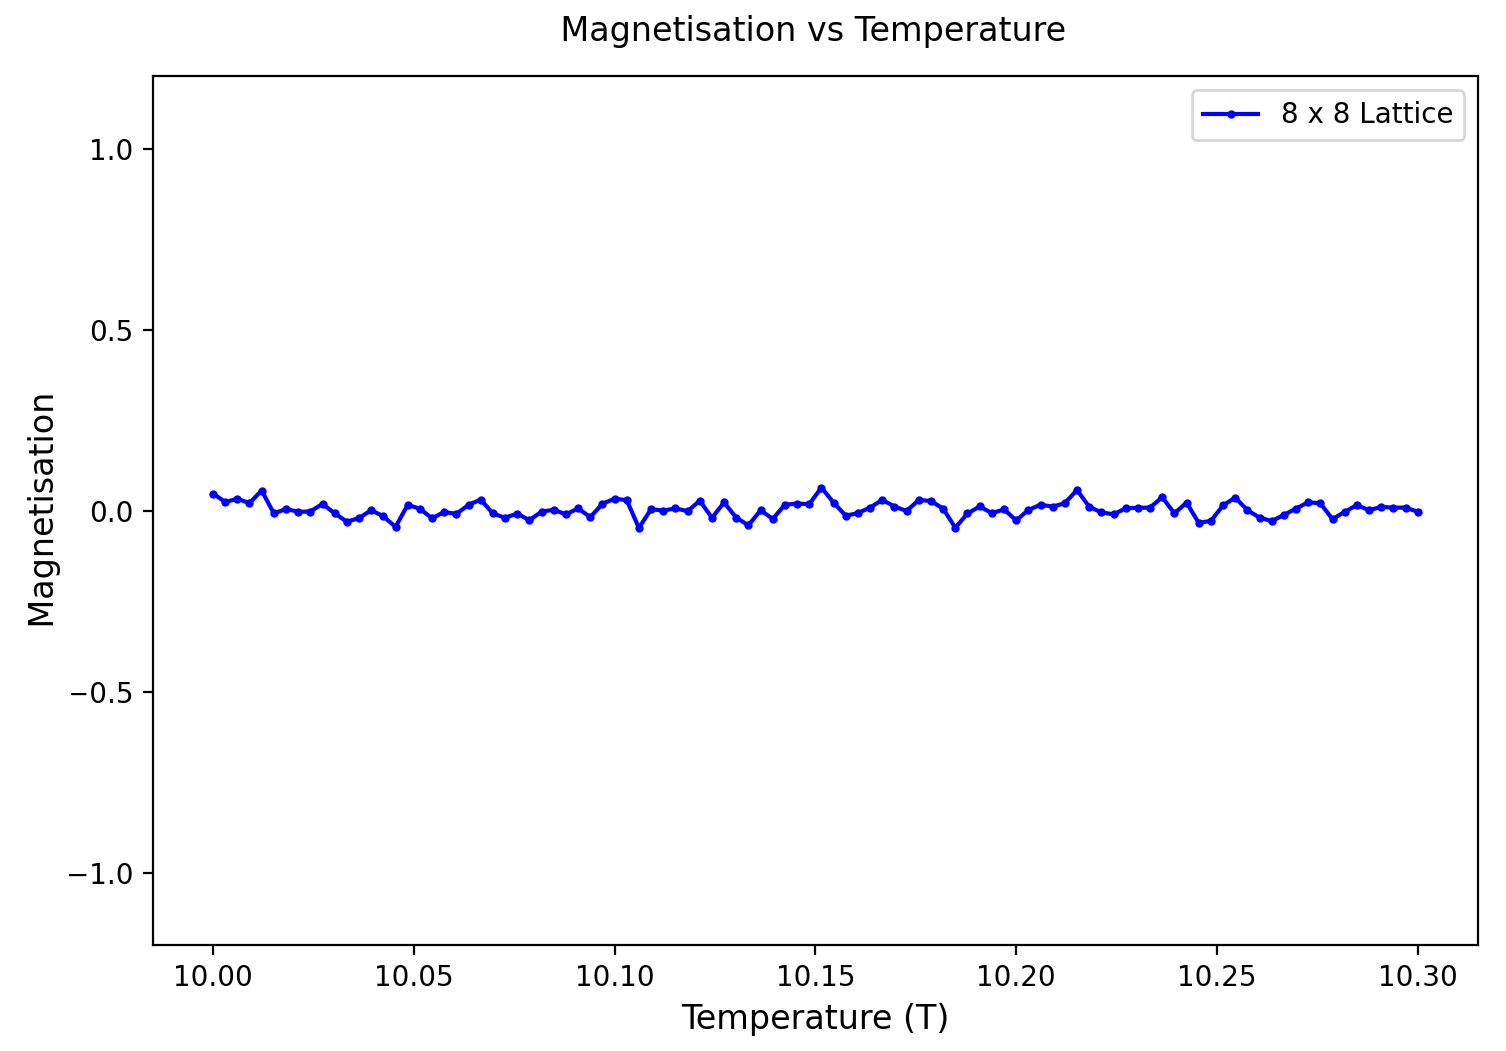
\includegraphics[width=1.1\linewidth,left]{mag vs temp high temp.png}
\caption{Magnetisation vs Temperature}
\label{fig:subim2}
\end{subfigure}
\caption{2D Ising Model at High Temperature}
\label{fig:image2}
\end{figure}

Similarly, the overall magnetisation of the system fluctuates around 0 which suggests that the system is paramagnetic; it has little or no influence by magnetism. This is reiterated through the lack of aligned spins in Figure 8(a). 

As a result of the high temperature, over time the system will be unable to reach equilibrium, regardless of how many Monte Carlo Metropolis simulations are run. When considering the Metropolis approach to simulating the Ising model, fixed temperatures below the critical temperature are often considered. Commonly, simulations are run with the temperature at a fixed rate of 0.4. 

\subsection{Simulating the 2D Ising Model Over Time}

We consider the 2D Ising model with energy defined in (2) and temperature, $T = 0.4$, exchange energy, $J = 1$, and Boltzmann constant $k_{B} = 1$. We will begin the system in a paramagnetic state and observe the system as it iterates through the Metropolis Algorithm (1.1).

\begin{figure}[!htb]
\minipage{0.32\textwidth}
  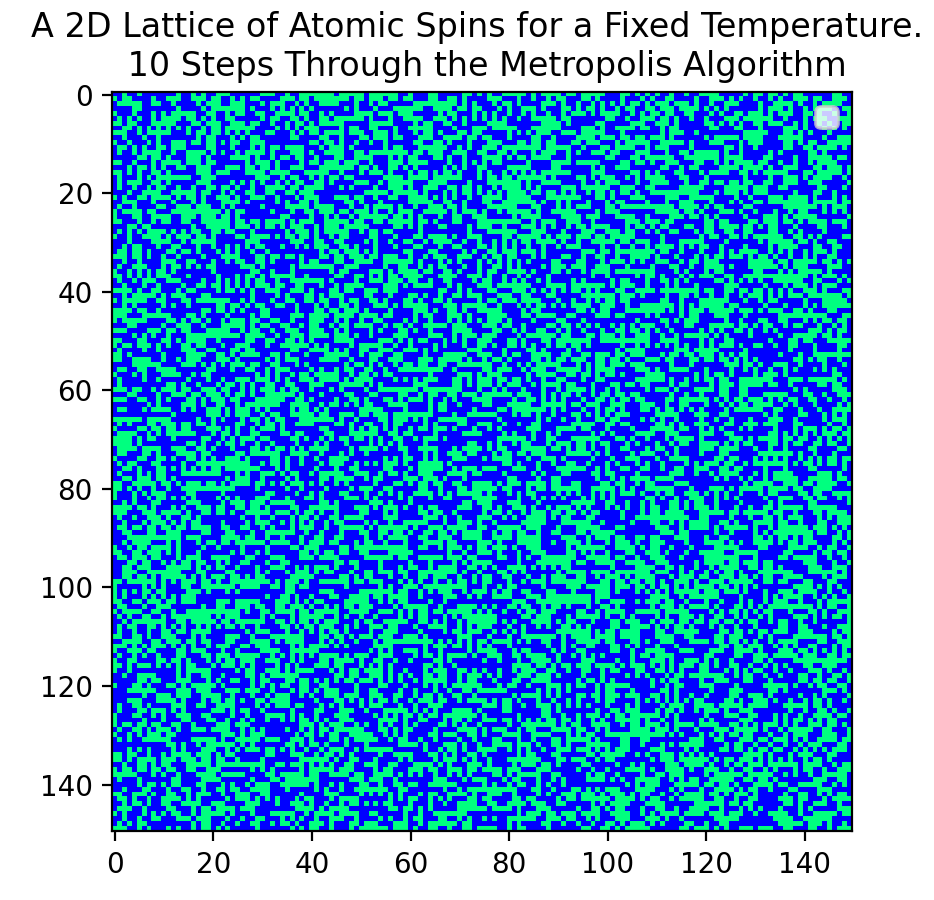
\includegraphics[width=\linewidth]{10 steps.png}
  \caption{10 Steps}\label{fig:10steps}
\endminipage\hfill
\minipage{0.32\textwidth}
  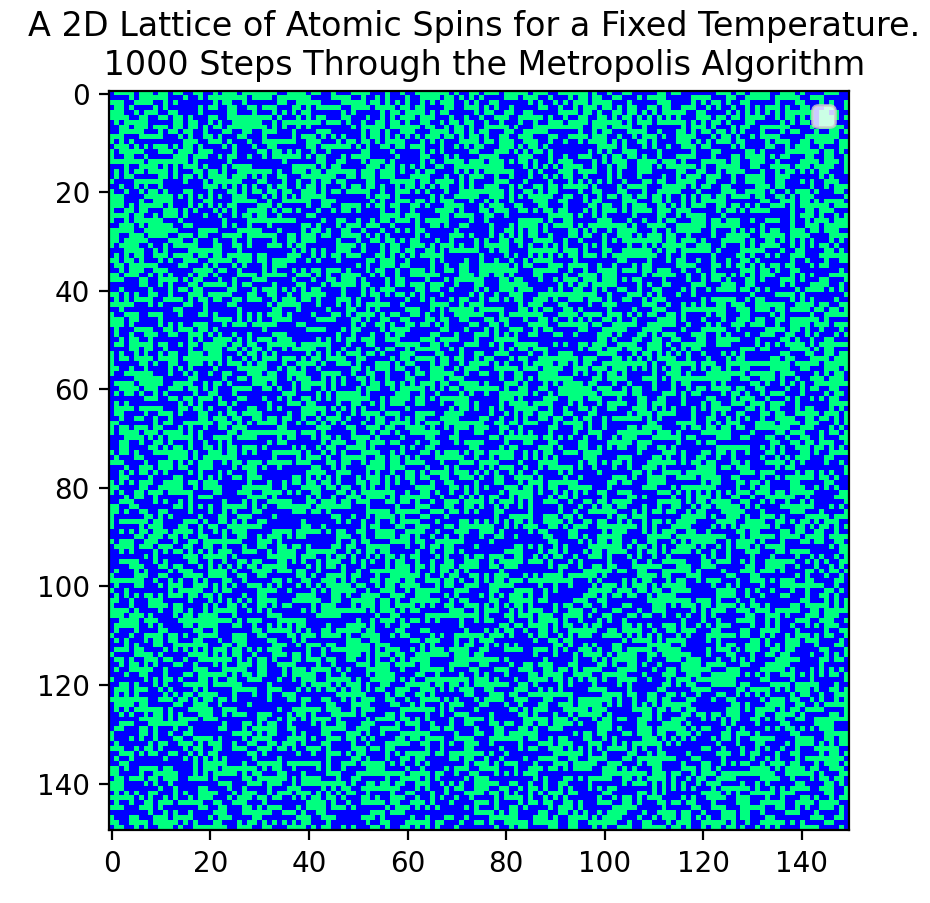
\includegraphics[width=\linewidth]{1000 steps.png}
  \caption{1,000 Steps}\label{fig:100steps}
\endminipage\hfill
\minipage{0.32\textwidth}%
  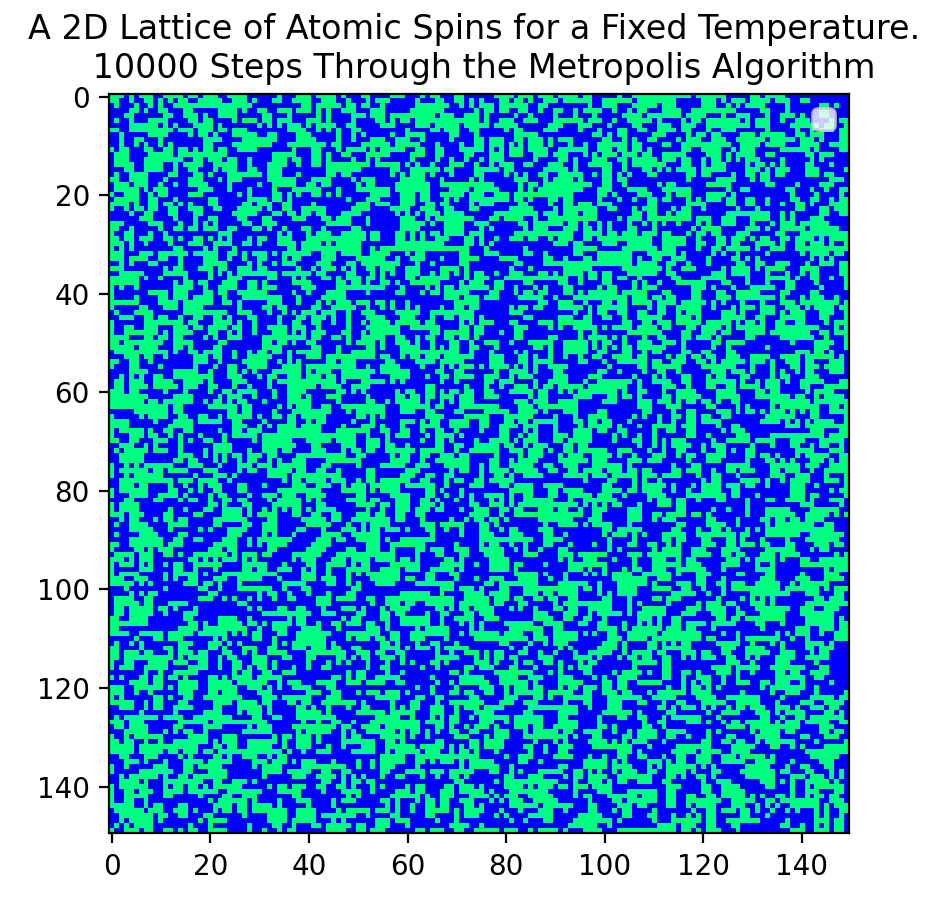
\includegraphics[width=\linewidth]{10,000 steps.png}
  \caption{10,000 Steps}\label{fig:1000steps}
\endminipage
\end{figure}

\begin{figure}[!htb]
\minipage{0.32\textwidth}
  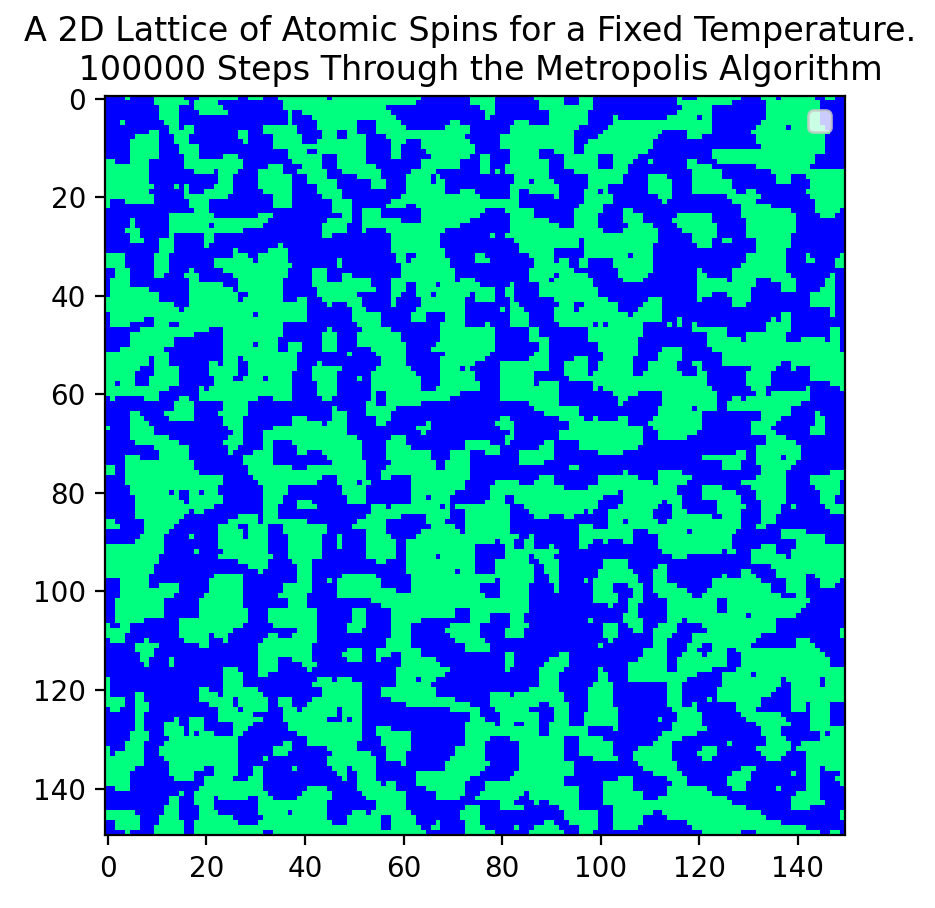
\includegraphics[width=\linewidth]{100,000 steps.png}
  \caption{100,000 Steps}\label{fig:10steps}
\endminipage\hfill
\minipage{0.32\textwidth}
  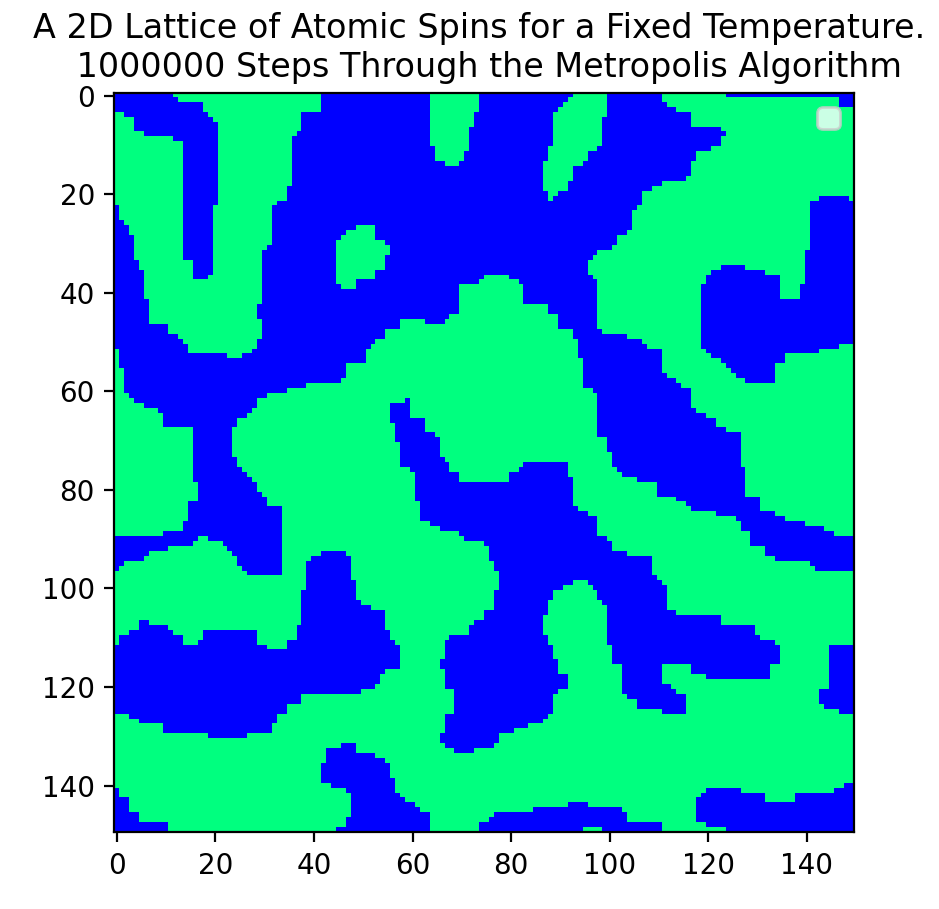
\includegraphics[width=\linewidth]{1,000,000 steps.png}
  \caption{1,000,000 Steps}\label{fig:100steps}
\endminipage\hfill
\minipage{0.32\textwidth}%
  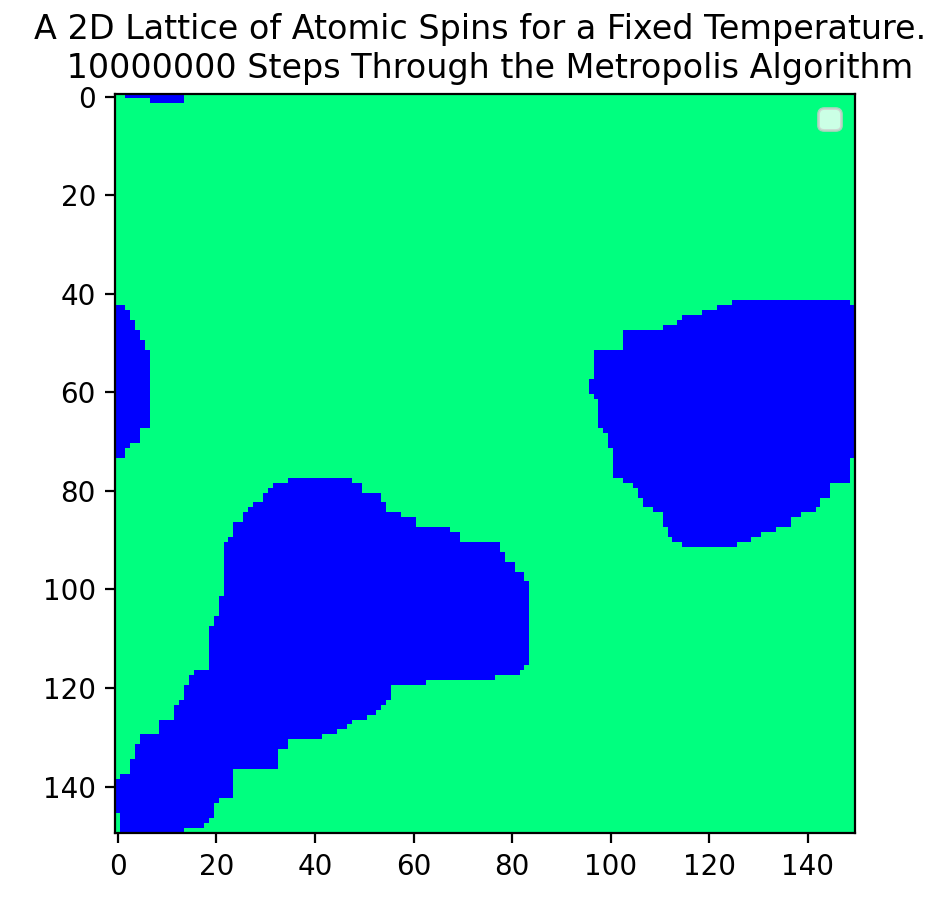
\includegraphics[width=\linewidth]{10,000,000 steps.png}
  \caption{10,000,000 Steps}\label{fig:1000steps}
\endminipage
\end{figure}

For a fixed temperature lower than the critical temperature, the disordered system tends towards an ordered, ferromagnetic system as it passes through increased steps of the Metropolis algorithm. 



%critical temperature has not been solved for any dimensions higher than 3d

%however, we can consider the 3d ising model and observe how the metropolis algoirthm allows the state to come to equilibrium.



%also add in about the magnetic field maybe?

%Move onto talk about the 3d case??

 

\section{References}
[1] \href{https://cds.cern.ch/record/2280218/files/cern-summer-student.pdf}{Some Reference}

\end{document}